%%%%%%%%%%%%%%%%%%%%%%%%%%%%%%%%%%%%%%%%%
% Professional Newsletter Template
% LaTeX Template
% Version 1.0 (09/03/14)
%
% Created by:
% Bob Kerstetter (https://www.tug.org/texshowcase/) and extensively modified by:
% Vel (vel@latextemplates.com)
% 
% This template has been downloaded from:
% http://www.LaTeXTemplates.com
%
% License:
% CC BY-NC-SA 3.0 (http://creativecommons.org/licenses/by-nc-sa/3.0/)
%
%%%%%%%%%%%%%%%%%%%%%%%%%%%%%%%%%%%%%%%%%

\documentclass[10pt]{article} % The default font size is 10pt; 11pt and 12pt are alternatives
\usepackage{lipsum,amsmath}
\usepackage[etex]{adjustbox}
\input{structure.tex} % Include the document which specifies all packages and structural customizations for this template

\begin{document}
\graphicspath{{../assets/img/}}
%----------------------------------------------------------------------------------------
%	HEADER IMAGE
%----------------------------------------------------------------------------------------

\begin{figure}[H]
  \centering\includegraphics[width=0.5\linewidth]{logo.png}
\end{figure}

%----------------------------------------------------------------------------------------
%	SIDEBAR - FIRST PAGE
%----------------------------------------------------------------------------------------

\begin{minipage}[t]{.30\linewidth} % Mini page taking up 30% of the actual page
  \begin{mdframed}[style=sidebar,frametitle={}] % Sidebar box

    %-----------------------------------------------------------

    \hypertarget{contents}{\textbf{{\large In This Issue\ldots}}} % \hypertarget provides a label to reference using \hyperlink{label}{link text}
    \begin{itemize}
    \item \hyperlink{message-sectionchair}{Message from incoming Section Chair, James Kimball} % These link to their appropriate sections in the newsletter
      %% \item \hyperlink{message-outgoingchair}{Message from outgoing Section Chair, Catherine Putnam}
    \item \hyperlink{message-sectionrep}{Message from Section Rep., Leigh Ann Myers}
    \item \hyperlink{sectionnext}{Message from the Section NExT Committee}
    \item \hyperlink{integrationbee}{2025 Integration Bee Results}
    \item \hyperlink{teamcompetition}{2025 Student Team Competition Results}
    \item \hyperlink{papercompetition}{2025 Student Papers Competition Results}
    \end{itemize}

    \centerline {\rule{.75\linewidth}{.25pt}} % Horizontal line

    \begin{enumerate}
    \item Mark your calendars! MathFest 2025 will be August 6-9, 2025 in Sacramento, CA.
    \item Join MAA!
    \end{enumerate}

    %-----------------------------------------------------------

    \textbf{Call for Volunteers!}

    \begin{itemize}
    \item \hyperlink{studentpaperscommittee}{Student Papers Committee}
    \item \hyperlink{locationcommittee}{Location and Nominations Committee}
    \item \hyperlink{nextcommittee}{Section NExT Committee}
    \item \hyperlink{teacherawardcommittee}{Outstanding Teacher Award Committee}
    \end{itemize}

    \textbf{Call for News!}
    Do you have news, announcements, or suggestions for the next newsletter?
    Send an email to the Communication Coordinator, Blake Farman, at \texttt{\mbox{bfarman@latech.edu}}

    %% \captionof*{table}{Table Caption}
    %% \begin{tabular}{llr}
    %%   \toprule
    %%   \multicolumn{2}{c}{Name} \\
    %%   \cmidrule(r){1-2}
    %%   First & Last & Grade \\
    %%   \midrule
    %%   John & Doe & $7.5$ \\
    %%   Richard & Miles & $2$ \\
    %%   \bottomrule
    %% \end{tabular}
  \end{mdframed}
\end{minipage}\hfill %
\begin{minipage}[t]{.66\linewidth} % Mini page taking up 66% of the actual page

  \hypertarget{message-sectionchair}{\heading{Message from Section Chair James Kimball}{6pt}} % \hypertarget provides a label to reference using \hyperlink{label}{link text}

  It was wonderful to see everyone at this year’s Louisiana-Mississippi Section Meeting at Belhaven University.
  Thank you to John Estes and his team for a great event.
  Over 120 students and faculty representing nearly 20 colleges and universities from across Louisiana and Mississippi attended the conference this year.
  We even had a group from The University of North Alabama pay us a visit.
  For those of you who were unable to attend, we had three amazing guest speakers.
  For our Anderson Lecture, Dr. James Tanton gave an engaging presentation on “The Bee Numbers.”
  %% Dr. Jenna Carpenter was our Section Visitor and led an insightful Section NExT Session for all faculty.
  Our Section NExT Session was led by both Dr. Tanton and Dr. Jenna Carpenter. 
  We were also blessed this year with a Polya Lecture from Dr. Pamela Harris on Multiplex juggling sequences and Konstant’s partition function.

  As always, the integration bee was a hit among the students.
  Thank you to Tilak for continuing this Section tradition.
  We had 11 student paper presentations and 13 Contributed Papers this year.
  The Student Paper Committee had a tough job with so many strong entries.
  Continue to encourage your students to pursue undergraduate research and scholarship and to present at the meeting.

  In light of the financial issues and budget constraints that every institution is facing, I am pleased that each of you make attending this conference a priority.
  Thank you for choosing this opportunity for you and your students.
  I believe this meeting, in particular, is the single best way to encourage ourselves and our undergraduate students to grow their appreciation and love for mathematics.
  I truly understand the sacrifice that some of you make to bring students to this meeting.
  Please encourage your colleagues to attend the meeting next year, which will be at The University of Louisiana at Lafayette.
  I hope to see everyone there.
  Also, please let me know if you plan to attend MathFEST 2025 in Sacramento, CA.
  We always go out to dinner as a group at MathFEST.

  As always, if you have any questions about anything or getting involved, please feel free to contact me.
  After all, it is the faculty and students that make each meeting special, meaningful, and memorable.  

  Jimmy Kimball\\
  University of Louisiana at Lafayette\\
  \texttt{james.kimball@louisiana.edu}

  
  %% In vel accumsan nisi. Sed eget justo a erat volutpat varius ut non quam. Nulla placerat eros id nibh laoreet pulvinar. Quisque semper.

  %% \begin{center}
  %%   \parbox[t]{.70\linewidth}{\textsl{Pellentesque gravida volutpat convallis. Ut sollicitudin egestas dictum. Pellentesque in nisi faucibus ullamcorper eu ac magna!}}
  %% \end{center}

  %% Duis eu \textsl{Felis eget}, purus bibendum elementum. Donec sed nunc sit amet ante congue aliquet tempus vitae ligula. Vestibulum dapibus malesuada purus, nec tincidunt lacus mollis ut. Nunc luctus accumsan tortor quis molestie. Donec erat nisl, auctor nec semper imperdiet, adipiscing ut ante. Vestibulum id metus libero, a vestibulum diam. 

  %% \begin{wrapfigure}[7]{l}[0pt]{0pt} % In-line figure with text wrapping around it
  %%   \includegraphics[width=0.3\textwidth]{placeholder.jpg}
  %% \end{wrapfigure}

  %% \textsl{Vivamus condimentum interdum} metus at varius vehicula, elit nunc sollicitudin enim, at scelerisque lorem urna vitae metus. Donec hendrerit consectetur tincidunt. Duis a magna justo. Nunc non mauris mi, eget commodo leo. Maecenas gravida lacus nunc, at viverra quam. Duis a turpis at lectus ultricies condimentum ut ut enim. Duis a magna justo. Nunc non mauris mi, eget commodo leo. Maecenas gravida lacus nunc, at viverra quam. Duis a turpis at lectus ultricies condimentum ut ut enim.

  %% Sed diam nisi, tristique ut dapibus a, volutpat vitae nisi. Vivamus aliquam quam sed mi rhoncus commodo. Suspendisse massa mauris, ullamcorper ut hendrerit vitae, ultrices eget ligula.

  %% Donec hendrerit consectetur tincidunt, nec gravida \href{http://www.example.com}{\textit{Duis a Magna Justo}} auctor nec, semper \href{http://www.example.com/}{Nec Gravida Rutrum} nulla nulla \href{http://www.example.com}{Elementum}, neque eu vulputate.

  %-----------------------------------------------------------

  %% \hypertarget{message-outgoingchair}{\heading{Message from outgoing Section Chair, Catherine Putnam}{6pt}} % \hypertarget provides a label to reference using \hyperlink{label}{link text}

  %% Aenean turpis libero, accumsan vitae sagittis eu, ornare eu lacus. Sed id odio eget velit congue porttitor. Cras quis neque non magna fringilla dapibus:

  %% \begin{itemize}
  %% \item morbi vulputate dapibus sapien
  %% \item cras vel nulla libero, in varius augue
  %% \item pellentesque quis nisl id 
  %% \end{itemize}

  %% Donec nulla elit, vulputate vel pharetra et, tempor ut nisl vivamus. Sapien lectus porttitor urna, sit amet lobortis odio eros at metus.

  %% Integer orci lorem, aliquam in dapibus at, tincidunt vitae felis nullam nec sem tellus, nec condimentum diam.

  %% Donec massa dolor, fermentum eget sagittis ut, sagittis placerat lacus. Donec id purus nunc fusce dignissim gravida condimentum. 

  %% Lorem ipsum dolor sit amet, consectetur adipiscing elit imperdiet vel pellentesque sed.

  %% Ut condimentum ornare rhoncus lorem ipsum dolor sit amet consectetu. Adipiscing elit \href{http://www.example.com}{Nunc Ultrices}.

\end{minipage} % End the main body - first page mini page

\begin{minipage}[t]{.95\linewidth}
  \begin{multicols}{2}
    \hypertarget{message-sectionrep}{\heading{Message from Section Rep., Leigh Ann Myers}{6pt}} % \hypertarget provides a label to reference using \hyperlink{label}{link text}
    It was great to see so many of you at the LA/MS Section Annual Meeting in Jackson.
    I hope you all (whether you made it to Jackson or not) will put next year’s meeting at University of Louisiana in Lafayette on your calendar.
    Before that, I hope to see you at MathFest this summer (August 6-9) in Sacramento, California.
    Please let me know if you plan to attend Math Fest.
    I will try to schedule a gathering for LA/MS Section members during Math Fest.
    This year’s MathFest will be the first for Jenna Carpenter, a former member of our section, as President of the MAA.
    It would be great to have a large turnout from Louisiana and Mississippi to support her.
    
    Please let me know if you have any concerns or questions about any MAA programs or if you have an interest in serving on a national committee.
    Also, be on the lookout for messages in our MAA Connect Community.
    I will post reminders about Math Fest plans through Connect.

    Leigh Ann Myers\\
    LA/MS Section Representative

    \BackToContents % Link back to the contents of the newsletter
    
    \hypertarget{sectionnext}{\heading{Message from the Section NExT Committee}{6pt}} % \hypertarget provides a label to reference using \hyperlink{label}{link text}

    First, I would like to thank the Section NExT committee members. They are: 

    \begin{itemize}
    \item
      Joshua Fontenot, University of Louisiana Lafayette
    \item
      Stacey McAdams, Louisiana Tech University
    \item
      Blake Farman, Louisiana Tech University
    \item
      Lee Dean, Delta State University
    \end{itemize}

    During the 2024 Fall semester, the Section NExT committee updated the Section NExT application process. Our goal was to encourage faculty to participate without adding undue work for them. As a result, the application consists only of a completed google document. We hope you will encourage any new faculty to participate in the Section NExT program. 

    For the Spring 2025 meeting we had five Section NExT Fellows participate in our program. These fellows are:

    \begin{itemize}
    \item
      Haile Gilroy, McNeese State University
    \item
      Phil Kains, Belhaven University
    \item
      Alissa Owens, Louisiana Tech
    \item
      Sarah Poiani, Mississippi University for Women
    \item
      Erasmus Tetteh-Bator, Jackson State University
    \end{itemize}

    We were delighted to have all three of the invited speakers participate in our section NExT program. Tanton talked about teaching transition courses. Jenna Carpenter participated virtually and talked about the benefits of MAA membership. We started off by having a 30 minute get to know you session where the fellows and committee members introduced themselves. We ended our morning sessions with a question-and-answer session where Fellows were able to ask questions and then have the group discuss.

    Traditionally Section NExT activities have taken place on Friday morning during the student competition. However, this year we asked the program chair if one of our speakers could speak on Friday afternoon. James Tanton gave a great talk about teaching general education courses. The Section NExT committee has plans to continue to offer programing for Section NExT Fellows both on Friday morning and throughout the conference.

    As we move into the 2025-26 academic year, we will need new members of the committee. If you are interested in working with this group to support the new faculty in our section, please reach out to Judith Covington at \texttt{covington@nsula.edu} or Section Chair Jimmy Kimball at \texttt{james.kimball@louisiana.edu}.

    \BackToContents % Link back to the contents of the newsletter
  \end{multicols}
\end{minipage}

\begin{minipage}[t]{.95\linewidth}
  \begin{multicols}{2}
    \begin{minipage}{\linewidth}
      \hypertarget{integrationbee}{\heading{2025 Integration Bee Results}{6pt}} % \hypertarget provides a label to reference using \hyperlink{label}{link text}
      This year marked the \(22^{\text{nd}}\) Anniversary of the Integration Bee.
      It has run continuously since 2004, with the inaugural event at Southeastern Louisiana University.
      Currently, it is led by Dr. Tilak de Alwis with help from Dr. Dennis Merino.

      \noindent\textbf{First Place:} \underline{Alameen Adeku}, Southeastern Louisiana University.

      \noindent\textbf{Second Place:} \underline{Dinesh Chhantyal}, University of\\ Louisiana at Monroe\\
      \textbf{Advisor:} Dr. Faisal Kaleem

      \noindent\textbf{Third Place:} \underline{Sumiksha Koirala}, University of Louisiana at Monroe\\
      \textbf{Advisor:} Dr. Faisal Kaleem
      
      \includegraphics[width=\linewidth]{integration_bee.png}\\
      %% Left to right: Dinesh Chhantyal, Alameen Adeku, Sumiksha Koirala
      
      \BackToContents % Link back to the contents of the newsletter
    \end{minipage}
    
    \begin{minipage}{\linewidth}
      \hypertarget{teamcompetition}{\heading{2025 Student Team Competition Results}{6pt}} % \hypertarget provides a label to reference using \hyperlink{label}{link text}
      \noindent\textbf{First Place:}
      \underline{Mississippi State University}\\
      Ryan Goodwin, Jonathan Kiesel, Kevin Ho, and Connor Doby\\
      \textbf{Advisor:} Ms. Jaclyn Smith

      \noindent\textbf{Second Place:}
      \underline{University of Louisiana at Lafayette}\\
      Jillian Michel, Michael Urny, Allison Zanyk, Scott Whitman\\
      \textbf{Advisor:} Dr. George Turcu

      \noindent\textbf{Third Place:}
      \underline{Louisiana Tech University}\\
      Clay Cook, Billy Deroche, Collyn Valentine, John Davis Vessel\\
      \textbf{Advisor:} Dr. Stacey McAdams
      
      \includegraphics[width=\linewidth]{team_comp-first_place.jpg}
      %% \includegraphics[width=\linewidth]{team_comp.jpeg}
      
      \BackToContents % Link back to the contents of the newsletter
    \end{minipage}
  \end{multicols}

  \hypertarget{papercompetition}{\heading{2025 Student Paper Competition Results}{6pt}} % \hypertarget provides a label to reference using \hyperlink{label}{link text}
  %% \begin{wrapfigure}[7]{l}[0pt]{0pt} % In-line figure with text wrapping around it
  %% \begin{wrapfigure}{r}{0.5\textwidth}
  %%   \vskip -\baselineskip% really top aligned
  %%   \includegraphics[width=\linewidth]{paper_comp.jpeg}
  %% \end{wrapfigure}
  \begin{adjustbox}{minipage=.5\textwidth,valign=T}
    \textbf{First Place:} Clay Cook, "Handle Number of Toroidal Graphs", Louisiana Tech University\\
    
    \textbf{Second Place:} Collyn Valentine, ``Explorations of Plane Graphs with No Odd Faces'', Louisiana Tech University\\
    
    \textbf{Third Place:} Nash Euto, ``Automated Scholarship Distribution Using Graph-Based Algorithms.'', Mississippi College  
  \end{adjustbox}\hfill
  \adjustimage{valign=T,width=.45\textwidth}{paper_comp.jpeg}\\
  
  
  \BackToContents % Link back to the contents of the newsletter
\end{minipage}

\begin{minipage}[t]{\linewidth}
  \hypertarget{volunteers}{\heading{Call for Volunteers}{6pt}}
  %% \begin{multicols}{2} % Two-column layout
    Our Section thrives on the energy and expertise of its members.
    Serving on a committee is a meaningful way to give back to the mathematics community, build professional relationships across the region, and help shape the direction of our programs and initiatives.

    Whether you’re passionate about mentoring new faculty, supporting students, recognizing outstanding teachers, or helping organize the annual meeting, there’s a place for your voice and your contributions.

    We are currently seeking volunteers for several standing committees.
    If you’ve been looking for a way to get more involved, we’d love to hear from you!
    
    \BackToContents % Link back to the contents of the newsletter

  %% \end{multicols}

  %----------------------------------------------------------------------------------------
  %	IN-TEXT BOX
  %----------------------------------------------------------------------------------------

  \begin{minipage}{.5\textwidth}
    \begin{mdframed}[style=intextbox,frametitle={}] % Sidebar box

      \hypertarget{studentpaperscommittee}{\heading{Student Papers Committee}{0pt}} % \hypertarget provides a label to reference using \hyperlink{label}{link text}
      The Student Papers Committee seeks a Chair and two members to help evaluate undergraduate and graduate student papers presented at our annual section meeting.
      The committee
      \begin{itemize}
      \item 
	Judges and awards prizes for student papers,
      \item
	Communicates results, and
      \item
        Facilitates professional development activities for students attending schools within the Section.
      \end{itemize}
      This is a wonderful opportunity to support and engage with emerging scholars across Louisiana and Mississippi.
      Members are eligible to serve multiple terms. Let us know if you’re interested in contributing to this rewarding work!
      \BackToContents % Link back to the contents of the newsletter

    \end{mdframed}%
  \end{minipage}
  \begin{minipage}{.5\textwidth}
    \begin{mdframed}[style=intextbox,frametitle={}] % Sidebar box

      \hypertarget{locationcommittee}{\heading{Location and Nominations Committee}{0pt}} % \hypertarget provides a label to reference using \hyperlink{label}{link text}
      We seek a Chair, one Louisiana member, and one Mississippi member to nominate leaders and organize meeting logistics.
      The committee 
      \begin{itemize}
      \item
        Nominates candidates for section offices,
      \item
        Assists the Chair in identifying and recruiting committee members,
      \item
	Announces the location and dates of the next annual meeting at the business session.
      \end{itemize}
      The Chair must be from the same state as the incoming Program Chair-Elect (this year, Mississippi).
      \BackToContents % Link back to the contents of the newsletter

    \end{mdframed}
  \end{minipage}
  \begin{minipage}{.5\textwidth}
    \begin{mdframed}[style=intextbox,frametitle={}] % Sidebar box

      \hypertarget{nextcommittee}{\heading{Section NExT Committee}{0pt}} % \hypertarget provides a label to reference using \hyperlink{label}{link text}
      The Section NExT (\textbf{N}ew \textbf{Ex}periences in \textbf{T}eaching) committee seeks two Mississippi members to recruit mentors and drive NExT programming.
      The committee
      \begin{itemize}
      \item
        Selects new Section NExT Fellows,
      \item
	Plans and facilitates Section NExT programming at the annual meeting.
      \end{itemize}
      Members serve alongside the Section NExT Coordinator, Judith Covington, and are eligible for multiple terms.
      If you’re eager to support new colleagues and strengthen our professional community, we’d love to have you join!
      \BackToContents % Link back to the contents of the newsletter

    \end{mdframed}
  \end{minipage}
  \begin{minipage}{.5\textwidth}
    \begin{mdframed}[style=intextbox,frametitle={}] % Sidebar box

      \hypertarget{teacherawardcommittee}{\heading{Outstanding Teacher Award Committee}{0pt}} % \hypertarget provides a label to reference using \hyperlink{label}{link text}
      The Outstanding Teaching Award Committee seeks one additional member to review nominations and help select this year’s award winner.
      \begin{itemize}
      \item
        The committee consists of five members, including the most recent awardee
      \item
        Appointed members serve two-year terms,
      \item
        Members review nominations and select the award winner, announced at the annual meeting.
      \end{itemize}
      This is a meaningful way to celebrate teaching excellence and elevate inspiring educators in our region. Nominate a colleague today!
      \BackToContents % Link back to the contents of the newsletter

    \end{mdframed}
  \end{minipage}

  %----------------------------------------------------------------------------------------
  %	QUOTATION
  %----------------------------------------------------------------------------------------

  %% \hypertarget{quotation}{{\large Quotes}} % \hypertarget provides a label to reference using \hyperlink{label}{link text}

  %% \begin{quote}
  %%   \textsl{``Praesent semper dui non justo rhoncus consequat. Mauris egestas tempus ligula, nec consequat arcu imperdiet eu. Mauris molestie lacinia enim, in dictum enim sagittis ac!!!!''} --- \textrm{John Smith}
  %% \end{quote}

  %----------------------------------------------------------------------------------------

\end{minipage}\vfill % End of the main body - second page mini page
%% \begin{minipage}[t]{.30\linewidth} % Mini page taking up 30% of the actual page

  %----------------------------------------------------------------------------------------
  %	SIDEBAR - SECOND PAGE
  %----------------------------------------------------------------------------------------

  %% \begin{mdframed}[style=sidebar,frametitle={}] % Sidebar box

  %%   \heading{Specifications}{0pt}

  %%   Magna ipsum:

  %%   \begin{enumerate}
  %%   \item Maecenas fringilla mi quis dolor vestibulum bibendum scelerisque erat rhoncus.
  %%   \item Ut id est metus, non pharetra leo Etiam in lorem sit amet sapien semper iaculis vel eget risus. Morbi consectetur gravida eros, non tincidunt ligula hendrerit vel.
  %%   \item Donec venenatis metus vitae urna malesuada vestibulum vitae eget mauris mauris sed orci dui, eget fringilla arcu. Nunc scelerisque tortor ut enim laoreet eget scelerisque ante ultricies.
  %%   \item Ut nec lacus vel ante molestie ac nec eros:

  %%     \textsl{Ipsum auctor} sit amet sapien semper.

  %%     \textsl{Eget fringilla} sed ut augue nec turpis vestibulum imperdiet.

  %%     \textsl{Tincidunt} ut id est metus, non pharetra leo.

  %%     \textsl{Vel velit venenatis } morbi consequat elementum eros, at pretium lectus gravida quis.

  %%     \textsl{Luctus nisi} morbi consectetur gravida eros, non tincidunt ligula hendrerit vel.

  %%     \textsl{Eget Odio} zunc scelerisque tortor ut enim laoreet eget scelerisque ante ultricie mollis lorem a sapien scelerisque varius.
  %%   \end{enumerate}

  %%   \BackToContents % Link back to the contents of the newsletter

  %% \end{mdframed}
  %% \hfill

  %----------------------------------------------------------------------------------------
\vfill
%% \centering
\hfill%
  \begin{minipage}[t]{.32\linewidth}
    \textbf{Contact Information:}\\
    Louisiana-Mississippi Section\\
    Mathematical Association of America\\
    %% 1234 Street Name,\\
    %% City, Country, Post Code\\
    \href{https://la-ms.maa.org}{https://la-ms.maa.org}\\
    \href{http://www.maa.org}{http://www.maa.org}\\
    %% \href{http://www.example.com}{http://www.nuncultrices.com} 
  \end{minipage}

  %----------------------------------------------------------------------------------------

%% \end{minipage} % End of the sidebar mini page

%% Photo collage
\begin{minipage}{\linewidth}
  \begin{center}
      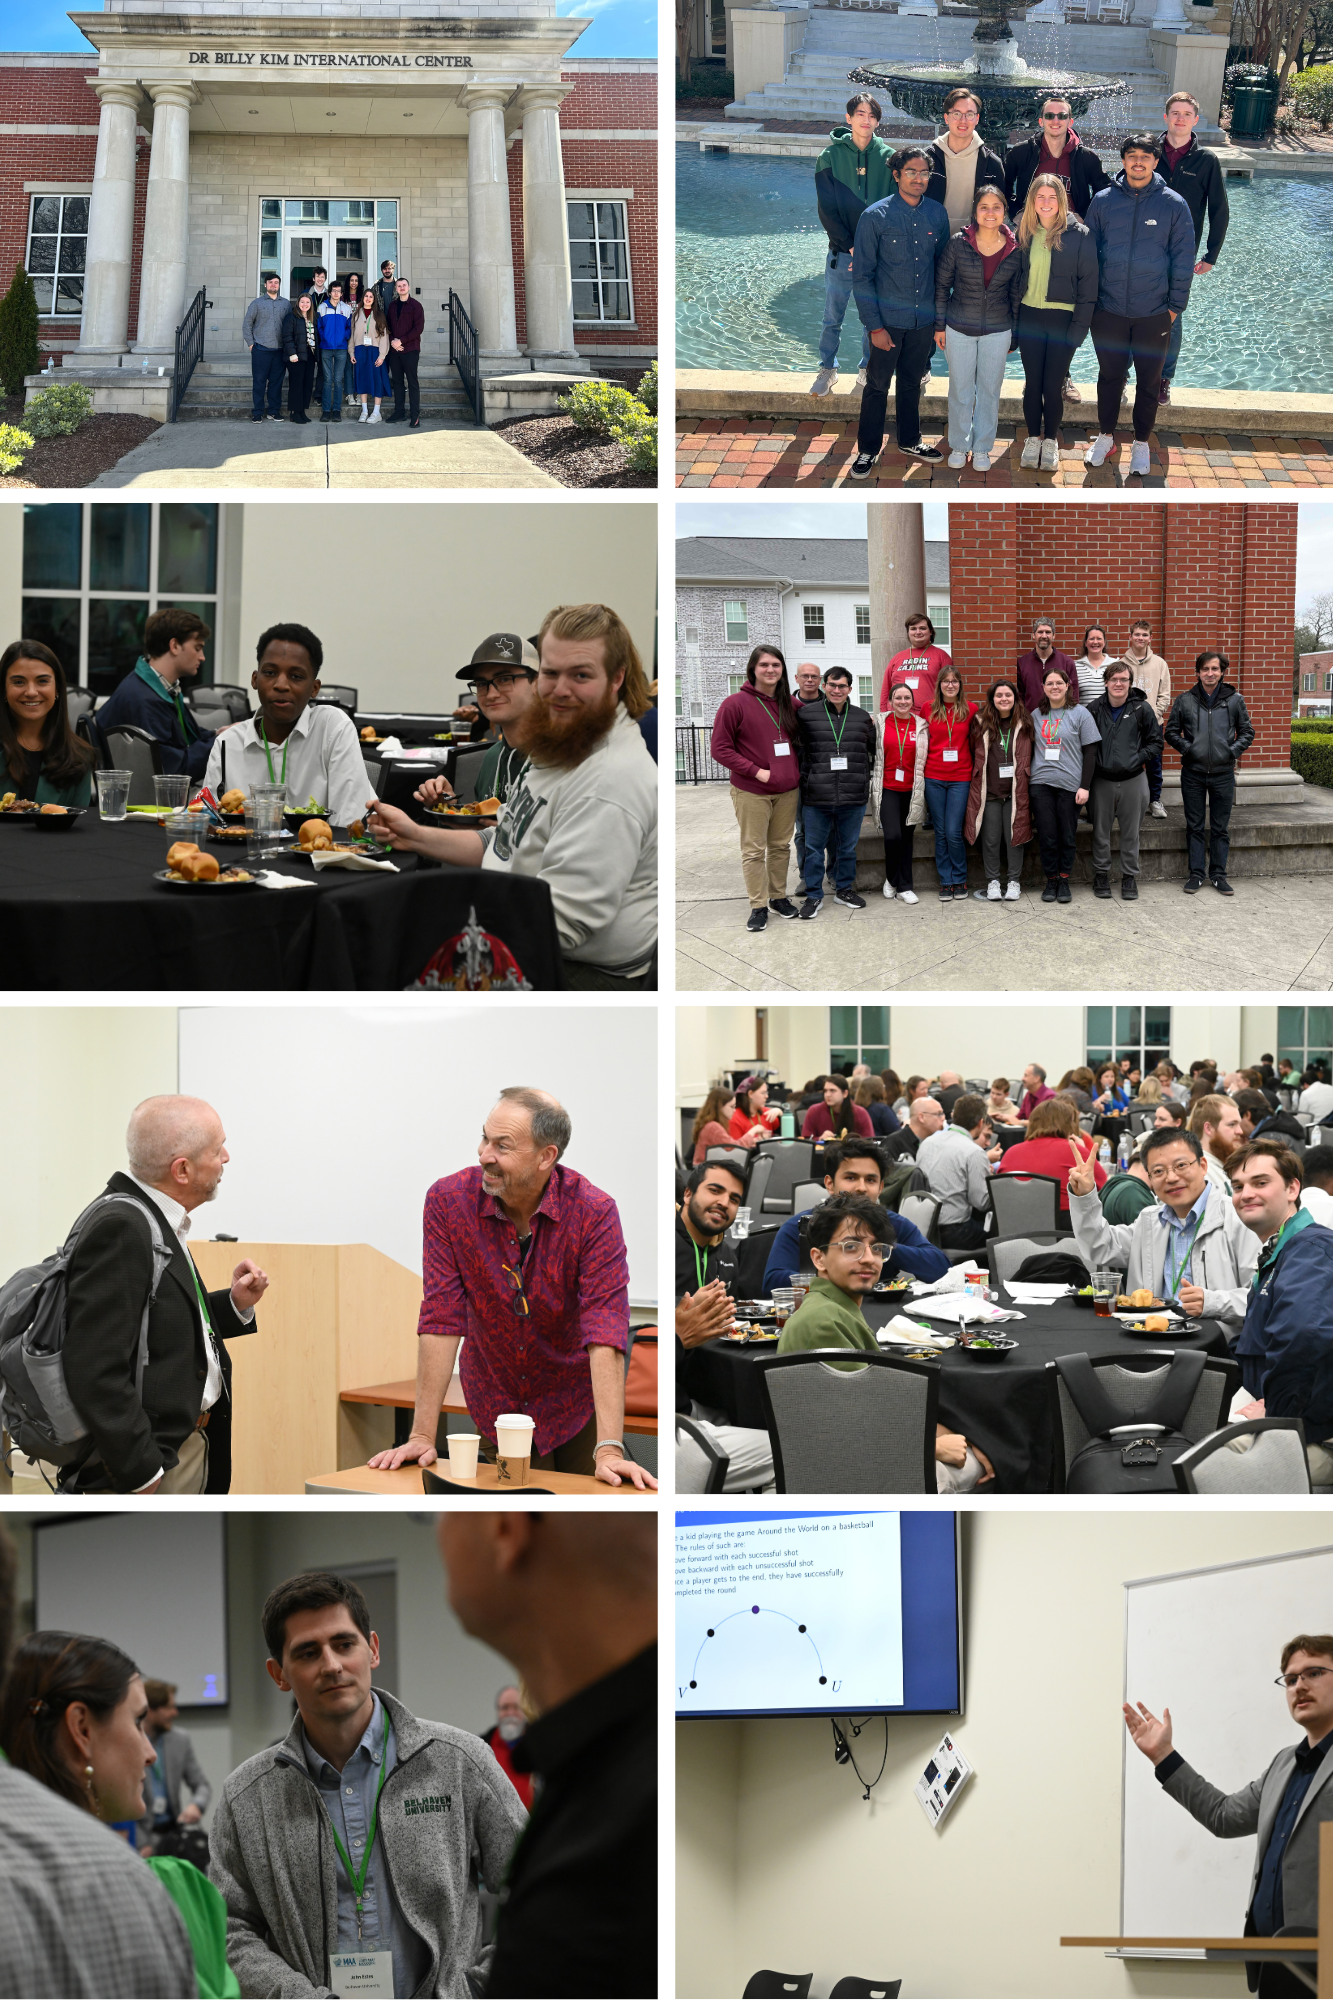
\includegraphics[width=.97\textwidth]{collage2.png}%
  \end{center}%
  \vfill
\end{minipage}
\end{document} 
